\documentclass{CSICC}
\usepackage{hyperref}
% تقریبا تمامی بسته‌های مورد نیاز برای یک مقاله در استایل فراخوانی شده است. اما در هر صورت در صورتی‌که می‌خواهید بسته‌ای را فراخوانی کنید به صورت زیر عمل کنید. مثلا ما در کد زیر دوبسته glossaries و tikz را فراخوانی کرده‌ایم.
%\makeatletter
%\bidi@BeforePackage{xepersian}{
%\RequirePackage{tikz}
%\RequirePackage{glossaries}
%}
%\makeatother


% عنوان مقاله را در این قسمت وارد کنید. 
\title{
خلاصه مقاله کنترل منبع:
سوء استفاده از سیستم های مدیریت کد منبع

}
\date{}
% اسامی نویسندگان و همچنین اطلاعات مربوط به آن‌ها را در این قسمت وارد کنید. 
\author[1]{برت هاوکینز}
\author[1]{بهاره کاوسی نژاد}
\author[2]{سیده شکیبا انارکی فیروز}
\affil[1]{
 دانشگاه علم و صنعت ایران، تهران
\lr{bahareh\_kavousi@comp.iust.ac.ir}
}
\affil[2]{
دانشگاه علم و صنعت ایران، تهران
\lr{shakiba\_anaraki@comp.iust.ac.ir}

}


\begin{document}
\maketitle
\begin{abstract}
	سیستم‌های مدیریت کد منبع (
	\lr{SCM}
	) نقش مهمی در سازمان‌ها دارند. این سیستم‌ها معمولاً برای مدیریت کد و ادغام با سایر سیستم‌ها در فرآیند
	 \lr{DevOps}
	  استفاده می‌شوند. اما، این سیستم‌ها نقاط ضعفی در برابر حملات زنجیره‌ی تأمین نرم‌افزار دارند و می‌توانند به مهاجمان امکان حرکت داخلی و افزایش دسترسی در سازمان را بدهند. این گزارش فنی به بررسی سیستم‌های
	   \lr{SCM}
	    معروف مانند 
	    \lr{GitHub Enterprise}
	    ، 
	    \lr{GitLab Enterprise}
	     و 
	     \lr{Bitbucket}
	      می‌پردازد و روش‌هایی را برای سوءاستفاده از آنها در حملات مختلف شامل بررسی، تغییر نقش کاربری، در اختیار گرفتن مخازن کد، جابه‌جایی به سیستم‌های دیگر، تقلید از کاربر و حفظ دسترسی پایدار توضیح می‌دهد. همچنین، ابزار
	       \lr{SCMKit}
	        تیم 
	        \lr{X-Force Red}
	         برای انجام این حملات استفاده می‌شود. در پایان، راهنمایی‌های دفاعی برای حفاظت از سیستم‌های
	          \lr{SCM}
	           نیز ارائه می‌شود.
\end{abstract}

\begin{keywords}
تجزیه و تحلیل کد منبع،
بررسی وابستگی،
کیفیت کد،
تست امنیت،
مدل سازی تهدید،
نظارت مستمر،
پاسخ حادثه،
\lr{DevSecOps}،
امنیت ابری.
\end{keywords}

\section{مقدمه}
سیستم های مدیریت کد منبع (
\lr{SCM}
) برای مدیریت کد منبع و تسهیل خط لوله
 \lr{DevOps}
  برای سازمان ها یکپارچه هستند. با این حال، این سیستم ها اغلب از نظر امنیت در مقایسه با سایر سیستم های سازمانی مهم مانند
   \lr{Active Directory}
    نادیده گرفته شده اند. سیستم های
     \lr{SCM}
     ، مانند
      \lr{GitHub Enterprise}
      ،
       \lr{GitLab Enterprise}
        و
         \lr{Bitbucket}
         ، به طور گسترده ای برای ذخیره و کنترل نسخه کد منبع، ادغام با ابزارهای مختلف، و امکان همکاری بین تیم های توسعه استفاده می شود.

در حالی که سیستم های 
\lr{SCM}
 مزایای متعددی را ارائه می دهند، خطرات امنیتی بالقوه ای را نیز به همراه دارند. مهاجمان می‌توانند از آسیب‌پذیری‌ها در این سیستم‌ها برای راه‌اندازی حملات زنجیره تامین نرم‌افزار، دسترسی غیرمجاز، و حرکت جانبی در زیرساخت‌های سازمان استفاده کنند. بهره‌برداری از سیستم‌های
  \lr{SCM} 
  می‌تواند منجر به عواقب شدیدی شود، از جمله اصلاحات غیرمجاز کد، سرقت مالکیت معنوی و به خطر افتادن سایر سیستم‌های
   \lr{DevOps}
    به هم پیوسته.

این مقاله با هدف روشن کردن اهمیت ایمن سازی سیستم های
 \lr{SCM} 
 و بررسی سناریوهای مختلف حمله ای که می تواند علیه پلتفرم های محبوب
  \lr{SCM}
   انجام شود را بررسی می کند. با درک این بردارهای حمله، سازمان ها بهتر می توانند در برابر تهدیدات احتمالی دفاع کنند. علاوه بر این، جعبه ابزار حمله مدیریت کد منبع
   \lr{ X-Force Red (SCMKit)} 
   معرفی خواهد شد که نشان می دهد چگونه می تواند این حملات را تسهیل و اجرا کند.

این مقاله موضوعات زیر را پوشش خواهد داد:



\begin{enumerate}
\item 
پیشینه سیستم های {SCM}\lr: مروری جامع بر سیستم های {SCM}\lr، هدف آنها و نقش آنها در اکوسیستم {DevOps}\lr.
\item
سناریوهای حمله: کاوش دقیق سناریوهای مختلف حمله، از جمله شناسایی، دستکاری نقش کاربر، تصاحب مخزن، چرخش به دیگر سیستم‌های {DevOps}\lr، جعل هویت کاربر، و حفظ دسترسی مداوم.
\item
بهره برداری از پلتفرم های محبوب {SCM}\lr: تجزیه و تحلیل عمیق آسیب پذیری ها و نقاط ضعف در سیستم های
 {SCM}\lr  
 پرکاربرد مانند
 \lr{GitHub Enterprise}
 ، 
 \lr{GitLab Enterprise}
  و 
  \lr{Bitbucket}
  .

\item 
مقدمه ای بر
 \lr{SCMKit}
 : مقدمه ای بر
  \lr{SCMKit X-Force Red}
  ، یک جعبه ابزار تخصصی که برای تسهیل و اجرای حملات علیه سیستم های SCM طراحی شده است.

\item 
راهنمایی دفاعی: توصیه‌ها و بهترین شیوه‌ها برای سازمان‌ها برای محافظت از سیستم‌های
 \lr{SCM}
  خود در برابر حملات احتمالی، از جمله ایمن کردن دسترسی کاربر، پیاده‌سازی مکانیزم‌های احراز هویت مناسب، نظارت بر فعالیت‌های مشکوک، و حفظ نسخه‌های نرم‌افزار به‌روز.
\end{enumerate}

با درک ریسک‌ها و اجرای اقدامات امنیتی مناسب، سازمان‌ها می‌توانند از یکپارچگی، محرمانه بودن و در دسترس بودن مخازن کد منبع خود اطمینان حاصل کنند، تأثیر احتمالی آسیب‌های سیستم
 \lr{SCM}
  را کاهش داده و از خطوط لوله
   \lr{DevOps}
    خود محافظت کنند.


\section{پیشنیازها}
\subsection{کنترل منبع در مقابل کنترل نسخه}
کنترل منبع و کنترل نسخه اصطلاحات نزدیک به هم هستند اما هدف‌ های کمی متفاوتی دارند. کنترل منبع به طور اختصاصی روی ردیابی تغییرات در کد منبع تمرکز دارد. کنترل نسخه فراتر رفته و شامل تغییرات در فایل‌ های باینری و انواع دیگر فایل‌ ها می‌شود. به عنوان مثال، کنترل نسخه می‌ تواند تغییرات را در فایل های کامپایل شده ردیابی کند، در حالی که کنترل منبع با تغییرات در کد منبع، مانند
 \lr{C\#}
  یا
   \lr{C++}
   ، که به تولید آن فایل های اجرایی‌ منجر شده‌ اند، سروکار دارد. نمونه ‌هایی از ابزارهای مورد استفاده در این زمینه‌ ها شامل
    \lr{Git}
    برای کنترل منبع و
     \lr{Subversion} 
     برای کنترل نسخه است.
\subsection{کنترل منبع در مقابل مدیریت کد منبع}
کنترل منبع شامل ردیابی تغییرات در کد منبع است. برای استفاده عملی در فرآیند توسعه، از سیستم ‌های مدیریت کد منبع (
\lr{SCM}
) استفاده می‌شود. سیستم‌ های 
\lr{SCM}
 ردیابی تغییرات را در مخازن کد منبع تسهیل می‌کنند و به توسعه ‌دهندگان در حل تعارضات هنگام ادغام همزمان کد از چندین مشارکت‌ کننده کمک می‌کنند.

\section{سیستم های مدیریت کد منبع(
\lr{Source Code Management Systems})
}
\subsection{بررسی اجمالی سیستم‌های
	 \lr{SCM}
	 }
سیستم‌ های
 \lr{SCM}
  به چندین عضو تیم اجازه می‌ دهند به طور همزمان روی همان فایل‌ های کد منبع کار کنند، تغییرات تاریخچه فایل‌ ها را ردیابی کرده و تعارضات را حل کنند. این سیستم ‌ها مجهز به رابط ‌های کاربری برای تعامل هستند و برای یکپارچگی قابل اعتماد در فرآیندهای توسعه ضروری‌ اند. سیستم‌ های
   \lr{SCM}
    محبوب شامل
     \lr{GitHub Enterprise}
     ،
      \lr{GitLab Enterprise}
       و
        \lr{Bitbucket}
         هستند که گزینه‌ های میزبانی متفاوتی ارائه می‌ دهند و از کنترل منبع
          \lr{Git}
           پشتیبانی می‌کنند. آن ‌ها همچنین با ادغام با سایر سیستم‌ ها، لوله‌کشی
            \lr{DevOps}
             را تسهیل می‌کنند.

\subsection{سیستم ‌های
	 \lr{SCM}
	  در لوله ‌کشی
	   \lr{DevOps}
	   }


در لوله‌کشی
 \lr{DevOps}
 ، سیستم‌ های
  \lr{SCM}
   در فاز ساخت، که تمام فازهای بعدی به کد منبع نگهداری شده در آن وابسته هستند، حیاتی هستند. پیشرفت از کد منبع به تولید شامل انتقال کد به یک سرور یکپارچه ‌سازی مداوم (
   \lr{CI}
   ) برای تست، اسکن و استقرار برای استفاده در تولید می‌شود.

\subsection{حملات زنجیره تامین نرم‌افزار}

این حملات، که اخیراًمحبوب شده اند، شامل تزریق کد مخرب توسط مهاجمان در فاز تولید است. این می ‌تواند منجر به سرایت گسترده در سازمان‌ های متعدد شود، همانطور که توسط نقض
 \lr{SolarWinds}
  نشان داده شده است. این سند به خطراتی که سیستم‌ های
   \lr{SCM} 
   در چنین حملاتی با آن مواجه هستند تأکید دارد.
   \subsection{حرکت جانبی به سایر سیستم‌های
   	 \lr{DevOps}
   	 }

سیستم ‌های
 \lr{SCM}
  می ‌توانند به عنوان نقطه دسترسی اولیه برای مهاجمان به منظور پیوست به سایر سیستم‌ ها در چرخه حیات
   \lr{DevOps}
   عمل کنند، مانند پلتفرم‌ های
    \lr{CI/CD} 
    یا مخازن بسته. مثال ‌ها شامل حرکت از سیستم
     \lr{SCM Bitbucket}
      برای سوء استفاده از سیستم ساخت
       \lr{Jenkins}
        یا از سیستم
         \lr{SCM GitLab Enterprise}
          به سیستم بسته‌بندی
           \lr{Artifactory}
            است. این سناریوها پتانسیل سیستم‌ های
             \lr{SCM}
              برای سوءاستفاده برای حملات بیشتر در زنجیره تامین نرم‌ افزار را برجسته می‌کنند.
\begin{figure}[t]
	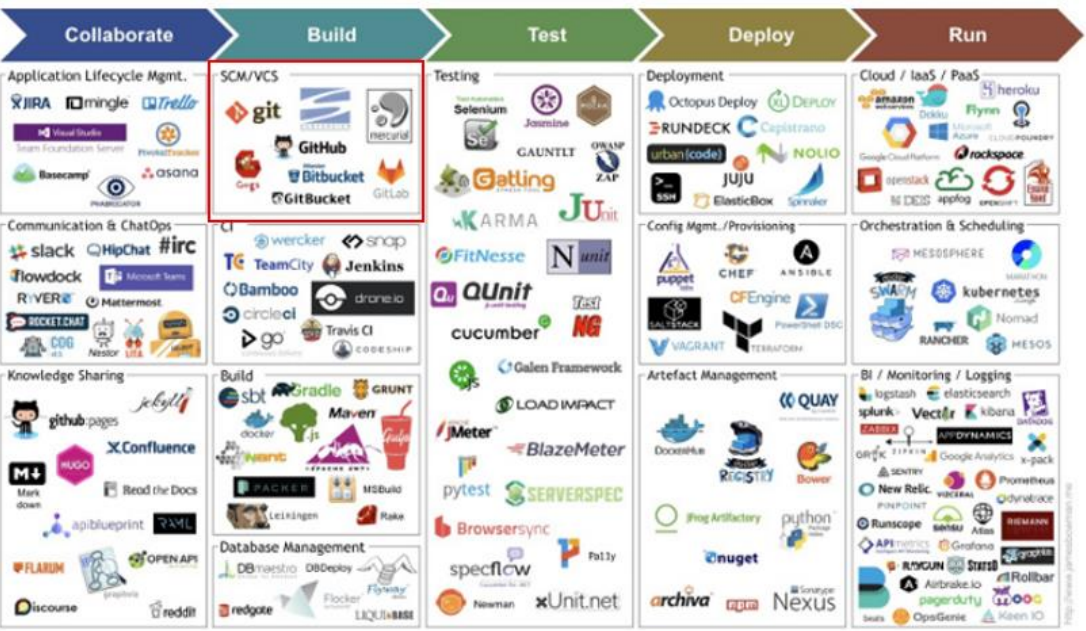
\includegraphics[width=.9\linewidth]{Images/Devops Pipeline Diagram}
	\caption{نمودار خط لوله 
	\lr{DevOps}
	}
	\label{fig:DevOps_Pipeline_Diagram}
\end{figure}


\section{
	\lr{Github Enterprise}
	}
	در
	 \lr{GitHub Enterprise}
	 ، استفاده از اصطلاحات "
	 \lr{enterprise}
	" و "
	 \lr{organization}
	 " مهم هستند. اصطلاح "
	 \lr{enterprise}
	 " به کل نمونه 
	 \lr{GitHub Enterprise} 
	 اشاره دارد. یک یا چندین سازمان می‌توانند در یک 
	 \lr{enterprise} 
	 قرار گیرند و 
	 \lr{enterprise} 
	 کلیه سازمان ‌ها را مدیریت می‌کند. لیست کاملی از اصطلاحات رایج استفاده شده در 
	 \lr{GitHub Enterprise} 
	 در
	  \href{ https://docs.github.com/en/enterprise-server@3.3/get-started/quickstart/github-glossary}{این منبع}
	   در دسترس است.
\subsection{سطوح دسترسی و نقش‌ها}
مالکان
 \lr{enterprise} 
 کلیه تنظیمات
  \lr{GitHub Enterprise}
  ، از جمله سازمان‌ها، تنظیمات و خط‌مشی ‌ها را مدیریت می‌کنند.
اعضابخشی از
\lr{enterprise}
  هستند و می‌توانند درون سازمان‌ ها کار کنند اما به تنظیمات سراسری
   \lr{enterprise} 
   دسترسی ندارند.
   \subsection{نقش‌ های سازمان}
مالکان سازمان تنظیمات و خط‌ مشی‌های سازمان را کنترل می‌کنند.
اعضای سازمان به پروژه‌ های درون سازمان کمک می‌کنند.
مدیران امنیت جنبه ‌های امنیتی پروژه‌ های سازمان را نظارت می‌کنند.
مدیران برنامه
 \lr{GitHub}
  ادغام و مدیریت برنامه ‌های
   \lr{GitHub}
    را انجام می‌دهند.
همکاران خارجی افرادی هستند که عضو سازمان نیستند اما برای همکاری در پروژه‌های خاص دسترسی داده شده‌اند.
\subsection{نقش‌های مخزن}
مجوز خواندن اجازه مشاهده و کلون کردن مخازن را بدون ایجاد تغییرات می‌دهد.
مجوز طبقه ‌بندی امکان مدیریت
 \lr{issue}
  و درخواست‌ های کشیدن(
  \lr{pull request}
  ) بدون دسترسی کامل را فراهم می‌کند.
مجوز نوشتن اجازه افزودن تغییرات به مخزن را می‌دهد.
مجوز نگهداری شامل دسترسی نوشتن به علاوه توانایی مدیریت تنظیمات مخزن است.
مجوز مدیریت کنترل کامل بر مخزن را ارائه می‌دهد، از جمله توانایی حذف یا انتقال مخزن.
\subsection{دامنه دسترسی توکن‌ها}
توکن‌های دسترسی در
 \lr{GitHub Enterprise}
  دارای “دامنه ‌های دسترسی" هستند که میزان دسترسی به ویژگی‌ های مختلف مانند مخازن، کلیدهای
   \lr{SSH} 
   و اطلاعات کاربر را تعریف می‌کنند و اطمینان از دسترسی امن و مناسب را فراهم می‌آورند.
\subsection{قابلیت‌های
	\lr{API}}   

\lr{API REST GitHub Enterprise }
امکان انجام مجموعه وسیعی از عملیات ‌ها مانند تعامل با مخازن، مدیریت توکن ‌های دسترسی، کلیدهای
 \lr{SSH}
  و انجام وظایف مدیریتی را فراهم می‌کند تا جریان‌ های کاری توسعه را ساده‌ سازی و خودکار کند.

\begin{table}[H]
	\centering
	\caption{جدول سناروهای جمله}
	\label{tab:Enterprise_attacks}
	\begin{tabular}{cp{5cm}}\hline
		سناریوی حمله
		& زیر-سناریو
		\\\hline
		% ---------------------------------
		شناسایی
		& 
		\begin{itemize}
			\item
			مخزن
			\item 
			فایل
			\item 
			کد
		\end{itemize}
		\\
		% ---------------------------------
		تصاحب مخزن
		& 
		نامشخص
		\\
		% ---------------------------------
		جعل هویت کاربر
		& 
		\begin{itemize}
			\item
			جعل ورود کاربر
			\item 
			جعل توکن
		\end{itemize}
		\\
		% ---------------------------------
		ارتقاء کاربر به ادمین سایت
		& 
		نامشخص
		\\
		% ---------------------------------
		حفظ دسترسی دائم
		& 
		\begin{itemize}
			\item
			توکن دسترسی شخصی
			\item 
			توکن جعل هویت
			\item 
			کلید 
			\lr{SSH}
		\end{itemize}
		\\
		% ---------------------------------
		دسترسی به کنسول مدیریت
		& 
		نامشخص
		\\
		\\\hline
	\end{tabular}
\end{table}

\section {\lr{GitLab Enterprise}}
\subsection{اصطلاحات}
یکی از اصطلاحات کلیدی که به طور مکرر در
 \lr{GitLab Enterprise }
 استفاده می‌شود، «پروژه ‌ها» است.
پروژه ‌ها می‌توانند کد را میزبانی کنند، مسائل را پیگیری کنند و می‌توانند حاوی خط لوله ‌های
 \lr{CI/CD} 
 باشند.

\subsection{مدل و سطوح دسترسی}
پنج نقش برای کاربر در زمینه مجوزهای پروژه در دسترس است که در زیر لیست شده‌اند:
\begin{itemize}
	\item مهمان
	\item گزارشگر
	\item توسعه‌دهنده
	\item نگهدارنده
	\item مالک
\end{itemize}
برای هر یک از پنج نقش، چندین مجوز عضو گروه در دسترس است.یک نکته قابل توجه این است که به طور پیش ‌فرض، کاربران می‌توانند نام کاربری خود را تغییر دهند و گروه‌ ها را ایجاد کنند.
هر نقش همچنین چندین مجوز خط لوله
 \lr{CI/CD}
  در دسترس دارد.
\subsection{دامنه ‌های توکن دسترسی}
مجموعا هشت دامنه توکن دسترسی شخصی در
 \lr{GitLab Enterprise}
  در دسترس است. لیستی از دامنه‌های مختلف و توضیحات آن‌ها در ادامه آمده است:
  \begin{table}[H]
  	\centering
  	\caption{ جدول دامنه های مختلف و توضیحات آن ها 	}
  	\label{tab:Domains}
  	\begin{tabular}{cp{5cm}}\hline
  		دامنه
  		& توضیحات
  		\\\hline
  		\lr{api}
  		&
  		خواندن-نوشتن برای کل
  		 \lr{API}
  		 ، شامل همه گروه‌ها و پروژه‌ها، رجیستری کانتینر و رجیستری بسته.
  		\\
  		%--------------------------------
  		\lr{read\_user}
  		&
  		خواندن فقط برای نقاط پایانی زیر
  		 \lr{/users}
  		 . به طور اساسی، دسترسی به هر یک از درخواست‌های 
  		 \lr{GET}
  		  در
  		   \lr{API}
  		    کاربران.
  		\\
  		%--------------------------------
  		\lr{read\_api}
  		&
  		خواندن فقط برای کل
  		 \lr{API}
  		 ، شامل همه گروه‌ها و پروژه‌ها، رجیستری کانتینر و رجیستری بسته.
  		\\
  		%--------------------------------
  		\lr{read\_repository}
  		&
  		خواندن فقط (
  		\lr{pull}
  		) برای مخزن از طریق
  		 \lr{git clone}
  		 .
  		\\
  		%--------------------------------
  		\lr{write\_repository}
  		&
  		خواندن-نوشتن (
  		\lr{pull, push}
  		) برای مخزن از طریق
  		 \lr{git clone}
  		 . لازم برای دسترسی به مخازن
  		  \lr{Git}
  		   از طریق
  		    \lr{HTTP}
  		     وقتی
  		      \lr{2FA}
  		       فعال است.
  		\\
  		%--------------------------------
  		\lr{read\_registry}
  		&
  		خواندن فقط (
  		\lr{pull}
  		) برای تصاویر رجیستری کانتینر اگر پروژه خصوصی است و احراز هویت لازم است.
  		\\
  		%--------------------------------
  		\lr{write\_registry}
  		&
  		خواندن-نوشتن (
  		\lr{push}
  		) برای تصاویر رجیستری کانتینر اگر پروژه خصوصی است و احراز هویت لازم است. (معرفی شده در
  		 \lr{GitLab 12.10}
  		 .)
  		\\
  		%--------------------------------
  		\lr{sudo}
  		&
  		اقدامات 
  		\lr{API}
  		 به عنوان هر کاربری در سیستم (اگر کاربر تأیید شده یک مدیر باشد).
  		\\

  		\\\hline
  	\end{tabular}
  \end{table}
  
 \subsection{قابلیت ‌های 
 	\lr{API}
 	}
 	\lr{API REST GitLab} 
 	به یک کاربر اجازه می‌دهد تا چندین عملیات مانند تعامل با پروژه‌ ها، توکن ‌های دسترسی، کلیدهای
 	 SSH
 	  و موارد دیگر را انجام دهد. این همچنین اجازه اقدامات اداری را می‌دهد.
 	مستندات کامل در مورد
 	 \lr{API REST}
 	  در 
 	  \href{https://docs.gitlab.com/ee/api/index.html}{اینجا}
 	   موجود است.
 	   
 	   \section{Bitbucket}
 	   یک نکته در مورد
 	   \lr{Bitbucket}
 	   این است که این پروژه به منظور نگهداری یک یا چندین مخزن طراحی شده است.
 	   \subsection{مدل و سطوح دسترسی}
 	   
 	   چهار سطح مجوز در
 	   \lr{Bitbucket}
 	   وجود دارد که شامل مجوزهای جهانی، پروژه، مخزن، و شاخه است. یک نکته قابل توجه این است که تمام مجوزها می‌توانند در سطح کاربر یا گروه تنظیم شوند. قبل از اینکه یک کاربر بتواند به
 	   \lr{Bitbucket}
 	   وارد شود، حداقل باید مجوزهایی در مجوزهای دسترسی جهانی به او اختصاص داده شده باشد.
 	   
 	   \begin{itemize}
 	   	\item دسترسی جهانی (
 	   	\lr{Global}
 	   	): 
 	   	تعیین می‌کند که چه کسی می‌تواند به Bitbucket وارد شود، چه کسی مدیر سیستم، مدیر و غیره است.
 	   	\item 
 	   	دسترسی پروژه (
 	   	\lr{Project}
 	   	): 
 	   	دسترسی‌های خواندن، نوشتن و مدیریت در سطح پروژه (گروه‌های مخازن).
 	   	\item 
 	   	دسترسی مخزن (
 	   	\lr{Repository}
 	   	):
 	   	دسترسی‌های خواندن، نوشتن و مدیریت بر اساس هر مخزن.
 	   	\item 
 	   	دسترسی شاخه (
 	   	\lr{Branch}
 	   	):
 	   	دسترسی نوشتن (
 	   	\lr{push}
 	   	) بر اساس هر شاخه.
 	   \end{itemize}
 	   
 	   
 	   
 	   در 
 	   \href{https://confluence.atlassian.com/bitbucketserver/global-permissions-776640369.html}{ اینجا
 	   }
 	   نقش‌های مختلفی که می‌توان از طریق \underline{دسترسی جهانی} اختصاص داد، توضیح داده شده است.
 	   
 	   در 
 	   \href{https://confluence.atlassian.com/bitbucketserver/using-project-permissions-776639801.html}{ اینجا
 	   }
 	   نقش‌های مختلفی که می‌توان از طریق \underline{دسترسی پروژه} اختصاص داد، توضیح داده شده است.
 	   
 	   
 	   در 
 	   \href{https://confluence.atlassian.com/bitbucketserver/using-repository-permissions-776639771.html}{ اینجا
 	   }
 	   نقش‌های مختلفی که می‌توان از طریق \underline{دسترسی مخرن} اختصاص داد، توضیح داده شده است.
 	   
 	   
 	   
 	   \lr{API REST Bitbucket}
 	   به کاربر اجازه می‌دهد تا اقدامات متعددی انجام دهد، مانند تعامل با پروژه‌ ها، مخازن، توکن ‌های دسترسی، کلیدهای
 	   \lr{SSH}
 	   و بیشتر. مستندات کامل درباره
 	   \lr{API REST}
 	   در
 	   \href{https://developer.atlassian.com/server/bitbucket/rest/v819/}{ این منبع
 	   }
 	   در دسترس است.
 \section{SCMKit}
 	در
 	 \lr{X-Force Red}
 	 ، ما خواستیم تا از قابلیت
 	  \lr{API REST}
 	   موجود در سیستم‌ های
 	    \lr{SCM}
 	     رایج دیده شده در تعهدات استفاده کنیم و قابلیت ‌های مفیدتری را در ابزاری به نام
 	      \lr{SCMKit}
 	       به صورت نمونه اولیه اضافه کنیم. هدف از این ابزار ارائه آگاهی از سوء استفاده از سیستم‌ های
 	        \lr{SCM}
 	         و تشویق به شناسایی تکنیک ‌های حمله علیه سیستم ‌های 
 	         \lr{SCM} 
 	         است.
 	\lr{SCMKit}
 	 به کاربر اجازه می‌دهد تا سیستم
 	  \lr{SCM}
 	   و ماژول حمله مورد استفاده را مشخص کند، همراه با مشخص کردن اعتبارنامه‌ های معتبر (نام کاربری/گذرواژه یا کلید
 	    \lr{API}
 	    ) به سیستم
 	     \lr{SCM}
 	      مربوطه. در حال حاضر، سیستم‌ های
 	       \lr{SCM} 
 	       که 
 	       \lr{SCMKit}
 	        پشتیبانی می‌کند شامل
 	        \lr{GitHub Enterprise}
 	        ،
 	        \lr{GitLab Enterprise}
 	          و
 	           \lr{Bitbucket Server}
 	            است. مهم ترین ماژول‌ های حمله پشتیبانی شده شامل شناسایی، افزایش امتیاز و پایداری هستند. ابزار و مستندات کامل در
 	            \href{https://github.com/xforcered}{
 	            	\lr{ GitHub X-Force Red}
 	            }
 	      موجود است.
 	      


\section{ملاحظات دفاعی}
در مقابله با سناریوهای مختلف حملات سایبری مانند شناسایی، جعل هویت کاربر، ارتقای کاربر به مدیر، حفظ دسترسی دائمی و تغییر خطوط لوله
 \lr{CI/CD}
 ، استراتژی‌های دفاعی برای
  \lr{GitHub Enterprise}
  ، 
  \lr{GitLab Enterprise}
   و
    \lr{Bitbucket}
    وجود دارد. توصیه‌ های کلیدی در این پلتفرم ‌ها عبارتند از:
\begin{itemize}
	\item
	نظارت و ثبت: اطمینان حاصل کنید که لاگ‌ های حیاتی برای تحلیل و تشخیص فعالیت‌ های مخرب به سیستم
	 \lr{SIEM} 
	 شما ارسال می‌شوند. این شامل لاگ‌ های حسابرسی، لاگ‌ های مدیریت، لاگ‌ های
	  \lr{API} 
	  و لاگ ‌های برنامه است.
	\item 
	تشخیص حمله: از فیلترهای جستجوی ارائه شده برای تشخیص سناریوهای حمله خاص با تجزیه و تحلیل لاگ ‌ها برای فعالیت‌ های غیرعادی مانند تلاش‌ های دسترسی غیرمجاز، جعل هویت کاربر و تغییرات در خطوط لوله
	 \lr{CI/CD}
	  استفاده کنید.
	\item 
	اقدامات پیشگیرانه: اقداماتی برای جلوگیری از حملات متداول را اجرا کنید، مانند غیرفعال کردن جعل هویت کاربر، تنظیم تاریخ انقضای خودکار برای توکن ‌های دسترسی شخصی و کلیدهای
	 \lr{SSH}
	، و نیازمندی به حداقل یک تاییدکننده برای هر کامیت کد. محدود کردن تعداد مدیران سایت یا سیستم و اجرای سیاست حداقل امتیاز نیز برای کمینه سازی سطوح حمله احتمالی توصیه می‌شود.
	\item 
	بهبودهای امنیتی: فعال‌ سازی احراز هویت چندفاکتوری (
	\lr{MFA}
	) برای دسترسی به این سیستم‌ های سازمانی، نیازمندی به امضای کامیت ‌ها با استفاده از کلیدهای
	 \lr{GPG}
	  یا گواهینامه‌ های 
	  \lr{S/MIME}
	  ، و اطمینان از حذف به موقع شاخه ‌های کد برای حفظ یک محیط تمیز و امن.
	\item
	دفاع از
	 \lr{SCMKit}
	: به طور خاص برای حملات مرتبط با 
	\lr{SCMKit}، نظارت بر امضاهای استاتیک، رشته ‌های عامل کاربر، و هر توکن دسترسی یا کلیدهای 
	\lr{SSH}
	 ایجاد شده با پیشوند "
	 \lr{SCMKit-}
	 " به عنوان نشانه ‌هایی از نفوذ پیشنهاد می‌شود.
\end{itemize}




این استراتژی ‌ها با هدف تقویت وضعیت امنیتی سازمان‌هایی که از GitHub Enterprise، GitLab Enterprise و Bitbucket استفاده می‌کنند، با ارائه بینش‌ های عملی برای شناسایی، پیشگیری و پاسخ مؤثر به تهدیدات سایبری طراحی شده‌ اند و به صورت مفصل تر در مقاله تشریح شده اند.

\section{نتیجه گیری}
سیستم های مدیریت کد منبع حاوی برخی از حساس ترین اطلاعات در سازمان ها هستند و جزء کلیدی در چرخه عمر
 \lr{DevOps}
  هستند. بسته به نقش یک سازمان، به خطر افتادن این سیستم ها می تواند منجر به سازش سایر سازمان ها شود. این سیستم‌ها برای یک مهاجم ارزش بالایی دارند و نیاز به دید بیشتری از سوی جامعه امنیت اطلاعات دارند، زیرا در حال حاضر در مقایسه با سیستم‌های دیگر مانند 
  \lr{Active Directory}
  ، بعدا اضافه شده اند. هدف
   \lr{X-Force Red} 
   این است که این مقاله و تحقیق توجه بیشتری را به خود جلب کند و الهام بخش تحقیقات آینده در مورد دفاع از این سیستم های سازمانی حیاتی باشد.

\section*{سپاس‌گزاری}
در پایان مقاله سپاسگزاری از این افراد به جهت کمک در بهبود مقاله بعمل آمده است:
\begin{itemize}
	\item \lr{Chris Thompson (@retBandit)}
	\item \lr{Daniel Crowley (@dan\_crowley)}
	\item \lr{Dimitry Snezhkov (@Op\_nomad)}
	\item \lr{Patrick Fussell (@capt\_red\_beardz)}
	\item \lr{Ruben Boonen (@FuzzySec)}
\end{itemize}

\section*{پیوست‌ها}
جدول زیر (
\ref{tab:attacks})
 سناریوهای حمله نشان داده شده در این مقاله را خلاصه می کند:
\begin{table}[H]
	\centering
	\caption{جدول سناروهای جمله
		\lr{SCM}
	}
	\label{tab:attacks}
	\begin{tabular}{cp{5cm}}\hline
		سیستم
		\lr{SCM}
		 & سناریو
		\\\hline
		\lr{GitHub Enterprise}
		&
		شناسایی
		\\
		\lr{GitLab Enterprise}
		&
		شناسایی
		\\
		\lr{Bitbucket}
		&
		شناسایی
		\\
		\lr{GitHub Enterprise}
		&
		حفظ دسترسی دائمی
		\\
		\lr{GitLab Enterprise}
		&
		حفظ دسترسی دائمی
		\\
		\lr{Bitbucket}
		&
		حفظ دسترسی دائمی
		\\
		\lr{GitHub Enterprise}
		&
		جعل هویت کاربر
		\\
		\lr{GitLab Enterprise}
		&
		جعل هویت کاربر
		\\
		\lr{GitHub Enterprise}
		&
		ارتقای کاربر به مدیر سایت
		\\
		\lr{GitLab Enterprise}
		&
		ارتقاء کاربر به نقش مدیر
		\\
		\lr{Bitbucket}
		&
		ارتقاء کاربر به نقش مدیر
		\\
		\lr{Bitbucket}
		&
		اصلاح خط لوله
		 \lr{CI/CD}
		\\
		\lr{GitLab Enterprise}
		&
		اصلاح خط لوله
		\lr{CI/CD}
		\\
		\lr{GitHub Enterprise}
		&
		تصاحب مخزن
		\\
		\lr{GitHub Enterprise}
		&
		دسترسی به کنسول مدیریت
		\\
		\lr{GitLab Enterprise}
		&
		دسترسی
		\lr{SSH}
		\\
		\\\hline
	\end{tabular}
\end{table}

%\bibliography{lib}
%\section*{مراجع}
%\href{https://www.blackhat.com/us-22/briefings/schedule/#controlling-the-source-abusing-source-code-management-systems-26423}
%hello.com
\section*{مراجع}
\begin{itemize}
	\item
	 \href{https://www.blackhat.com/us-22/briefings/schedule/#controlling-the-source-abusing-source-code-management-systems-26423}{برنامه جلسات توجیهی 
	 	\lr{Black Hat USA 2022}
	 	}
\end{itemize}

\end{document}


